% \newcommand{\prototitle}{Versuch 2 - Statistik}
% \newcommand{\Fachbereich}{Praktikum Messtechnik}
% \input{../packages/tu_header}

\newcommand{\institut}{Institut f\"ur Telekommunikationssysteme}
\newcommand{\fachgebiet}{Nachrichten\"ubertragung}
\newcommand{\veranstaltung}{Praktikum Nachrichten\"ubertragung}
\newcommand{\pdfautor}{\"Ozg\"u Dogan (326 048), Boris Henckell (325 779)}
\newcommand{\autor}{\"Ozg\"u Dogan (326 048)\\ Boris Henckell (325 779)}
\newcommand{\gruppe}{Gruppe: D03}
%\newcommand{\betreuer}{Betreuer: Mahmoud Felk}


\newcommand{\pdftitle}{Nachrichten\"ubertragung\ Praktikum\ 04}
\newcommand{\prototitle}{Praktikum 04 \\ Pulsamplitudemodulation und nichtideale Abtastung}


\input{../../packages/tu_header_8}
%\begin{document}

% \lstlistoflistings
\definecolor{darkgray}{rgb}{0.95,0.95,0.95}
\definecolor{darkolivegreen}{HTML}{01a801}
\definecolor{functionsBlue}{HTML}{32b9b9}
\definecolor{variableRed}{rgb}{1,0,0}
\definecolor{stringBrown}{HTML}{bc8e8e} % f geht nicht

\lstset{
        %\lstset{extendedchars=true} % Umlaute an der richtigen stelle und nicht am Anfang ausgeben
        %basicstyle=\footnotesize\ttfamily,
        basicstyle=\small,
        %
        inputencoding=utf8,
        %
        tabsize=4,
        showspaces=false,
        showtabs=false,
        showstringspaces=true, % no special string spaces
        %
        backgroundcolor=\color{darkgray}, % background
        stringstyle=\color{stringBrown}\fseries, % Strings
        keywordstyle=\color{functionsBlue}\bfseries, % keywords Blau
        identifierstyle=\color{variableRed}, % variablen
        commentstyle=\color{darkolivegreen}, %  comments
        %
        breaklines=true,
        %
        numbers=left,
        numberstyle=\tiny,
        stepnumber=1,
        numbersep=7pt,
        %
        frame=single,
        columns=flexible,
        %
        xleftmargin=-2cm,
        xrightmargin=-1.5cm,
        %
        language=Matlab
}

%---------------------------------------------------------------------
%---------------------------------------------------------------------
%---------------------------------------------------------------------


\section{Einleitung}
\begin{quote}
	\TODO{Einleitung so okay?}
	In diesem Termin werden zwei nichtideale Abtastverfahren für die
	Rekonstruktion eines PAM-modulierten Signals untersucht. Diese zwei Verfahren
	sind die Abtastung durch Signalausblendung (shape-top sampling) und die
	Abtastung mit Signalverbreiterung (flat-top sampling). Beide Verfahren werden
	im Zeit- und im Frequenzbereich untersucht, dabei werden ihre Auswirkungen auf
	die Rekonstruktion der abgetasteten Signale interpretiert.
\end{quote}%beende Einleitung
%--------------------------------------------------------------------
%--------------------------------------------------------------------    


\section{Theorie}
\begin{quote}
	\subsection{Abtastung durch Signalausblendung (shape-top sampling)}
    \begin{quote}  
        \TODO{Theorie einfügen}
        
    \end{quote}
    
    \subsection{Abtastung mit Signalverbreiterung (flat-top sampling)}
    \begin{quote}
    	\TODO{Theorie einfügen}
    \end{quote}

    
    \subsection{Vorbereitungsaufgabe}
    \begin{quote}        
        Zunächst werden die Formeln für das Spektrum eines abgetasteten Signals
        hergeleitet. Das $\alpha$ steht dabei für das Tastverhältnis.
        
        \subsubsection{Shape-Top-Sampling}
        \begin{quote}
            \begin{equation*}
                \begin{split}
                    f_m (t)   &= f(t) \cdot \sqcap_{\alpha T} (t) \ast \delta_T (t) \\
                    F_S (j\omega) &= \frac{1}{2\pi} F (j\omega) \ast \left [
                    \alpha T \cdot si \left( \frac{\omega \alpha T}{2} \right) \cdot \omega_T \cdot \delta_{\omega T} (\omega) \right] \\
                    &= \alpha \cdot F (j \omega) \ast \left ( si \left( \frac{\omega \alpha T}{2} \right)
                    \sum_{k=-\infty}^{\infty} \delta (\omega - k\omega_T) \right)\\
                    &= \alpha \cdot F (j \omega) \ast \sum_{k=-\infty}^{\infty} (si(k \pi \alpha) \cdot \delta (\omega -
                    k\omega_T))\\
                    &= \alpha \cdot \sum_{k=-\infty}^{\infty} \left [ si(k \pi \alpha) \cdot F (j(\omega - k\omega_T))
                    \right]\\
                \end{split}
            \end{equation*}
        \end{quote}
        
        \subsubsection{Flat-Top-Sampling}
		\begin{quote}
			\begin{equation*}
            	\begin{split}
            		f_m (t) &= [f (t) \cdot \delta_T (t)] \ast \sqcap_{\alpha T} (t)\\
            		F_F (j\omega) &= \left ( \frac{1}{2 \pi} F (j\omega) \ast \omega_T
            		\cdot \delta_T (\omega) \right) \cdot \alpha T \cdot si (\frac{\alpha \omega T}{2})\\
            		&= \alpha \cdot si \left( \frac{\omega \alpha T}{2} \right) \cdot \sum_{k=-\infty}^{\infty} F(j(\omega -
            		k\omega_T))\\
            	\end{split}
            \end{equation*}
		\end{quote}
		
		Danach werden die resultierenden Spektren $F_S (j\omega)$ und $F_F (j\omega)$
		für das Nutzsignal
		\begin{equation*}
        f(t) = A \cdot cos(\frac{\omega_T}{5}t)    	
        \end{equation*}
		mit $\alpha = 0.5$ und $\omega_T = 20\pi kHz$.
		
		
		 \begin{figure}[H]
    \centering
        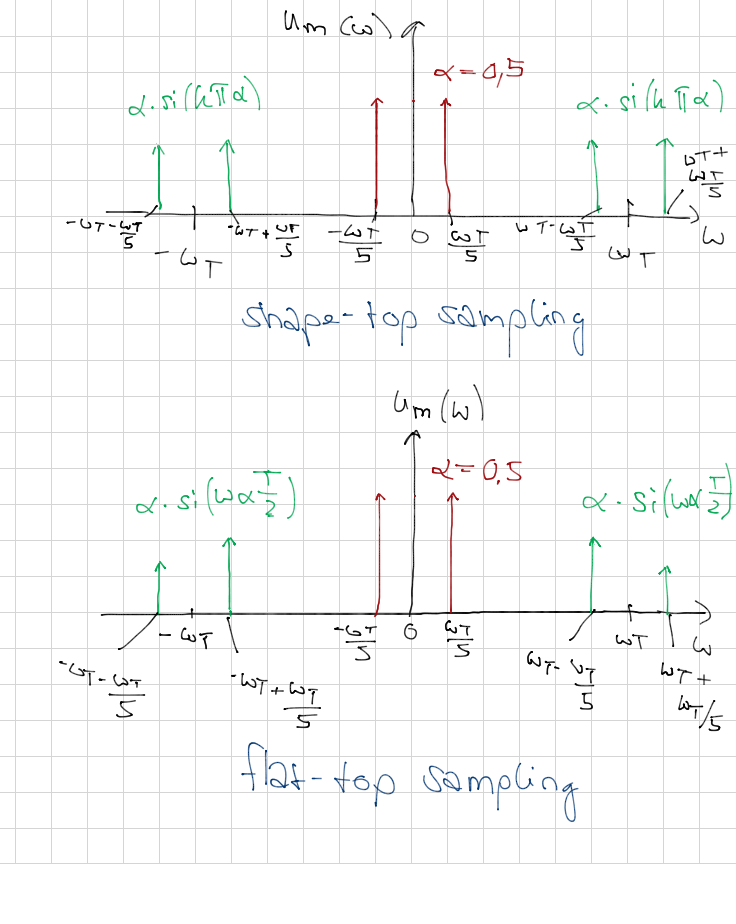
\includegraphics[scale=0.3, trim = 0cm 0cm 0cm 0cm,
        clip]{./Bilder/vorbereitungsskizze}
            \caption{Skizze}
  	    \end{figure}
		
		Es ist zu sehen, dass sich die Amplituden der Spektren mit einem
		Si-Funktionsfaktor, welcher von dem eingesetzten $\alpha$ abhängt, verringern.
		Bei der shape-top Abtastung ist dieser Faktor unabhängig von der Frequenz
		$\omega$. Daher sind die Amplituden der Peaks, die an den Grenzen eines
		Frequenzbandes entstehen, immer gleich groß.    	
		Bei der flat-top Abtastung ist dieser Faktor sogar von der Frequenz abhängig, daher entsteht 
		eine Amplitudenverringerung von zwei Peaks an den Rändern eines
		Frequenzbandes.\\
		Mit $\alpha$ gegen $0$ geht auch die Amplitude des Basisbands (k = $0$) gegen
		$0$. Somit werden alle folgenden Peakamplituden (deren Amplituden sich bei der
		shape-top Abtastung mit $\alpha \cdot si(k \pi \alpha)$ und bei der flat-top
		Abtastung mit $\alpha \cdot si(\frac{\omega \alpha T}{2})$ bilden) ebenfalls
		verschwindend gering. ist das $\alpha$ aber $1$, beträgt die Amplitude des
		Basisbands $1$ und die folgenden Peakamplituden lassen sich wie bereits
		erwähnt berechnen.
    	
    	\TODO{Ist das okay so Boris?}
    	
    	Außerdem wird die Planung zur Praktikumsdurchführung im voraus gemacht. Für
    	den Versuch haben wir uns folgendes überlegt\ldots
    	\TODO{Stichwortartige Beschreibung über die Realisierung des Aufbau,
    	Blockschaltbilder einfügen, erwähnen wo wichtige Messungen gemacht werden
    	sollen}
    	
    	.
    	.
    	.
    	
    	Zuletzt wird eine MATLAB-Simulation der Abtastung mittels Signalausblendung
    	und Signalverbreiterung für ein Sinussignal als Quellsignal und der
    	Abtastfrequenz von $400 kHz$ ausgeführt. Das verwendete Quellsignal
    	hatte eine Amplitude von $2V$ und eine Frequenz von $2 kHz$. Das
    	Abtastrechtecksignal hatte eine variable Frequenz ($10 kHz und 20 kHz$),
    	eine variable Amplitude (gewählt haben wir $1V, 2V$ und $3V$) und ein
    	variables Tastverhältnis von $0.2, 0.5$ oder $0.7$.\\
    	Für den hiesigen Vergleich haben wir nur die Abtastamplituden $1V$ udn $3V$
    	verwendet.
    	
    	Zuerst betrachten wir die Simmulationsergebnisse der Abtastung durch
    	Signalausblendung:
    	
    	 \begin{figure}[H]
        \centering
        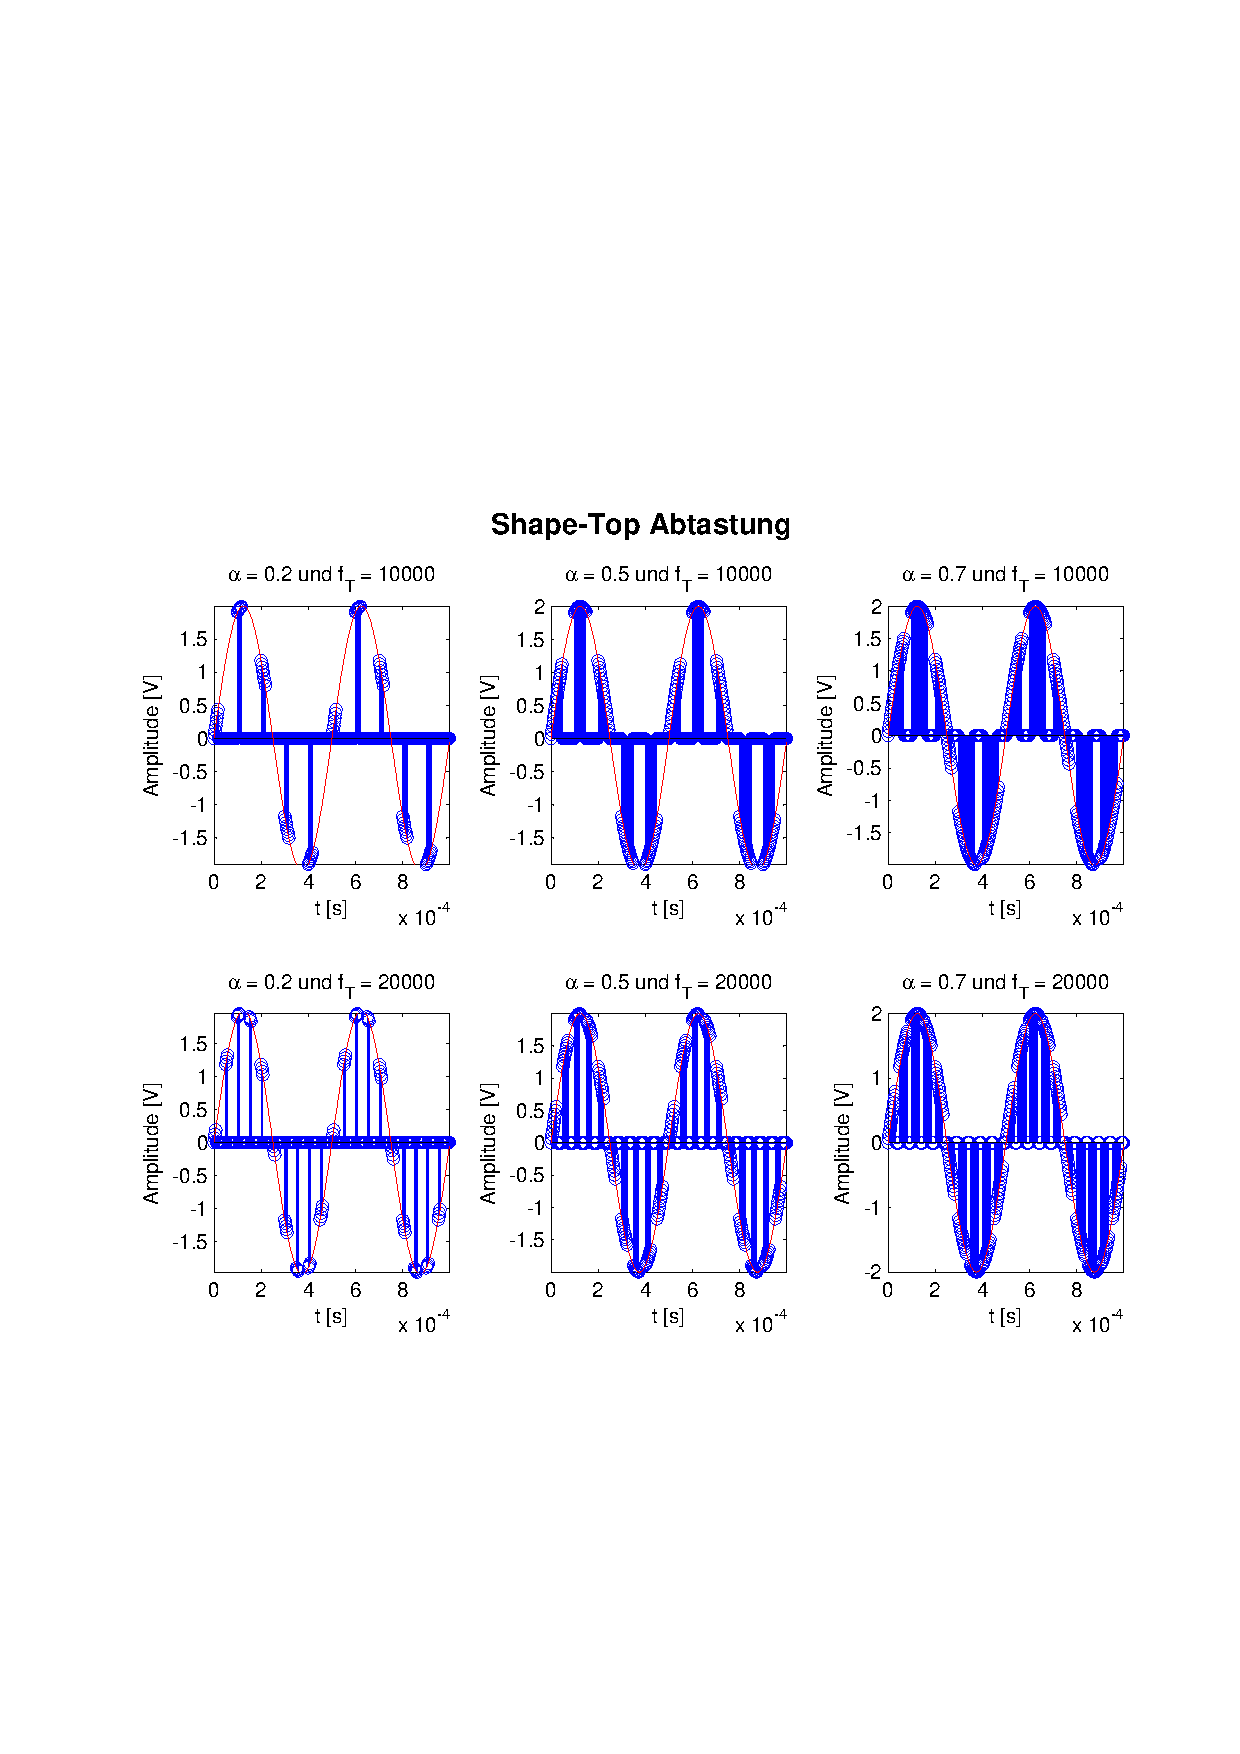
\includegraphics[scale=0.7, trim = 1.5cm 6cm 1cm 8cm,
        clip]{./Bilder/shape-top-zeit_1V}
            \caption{Zeitsignal mit shape-top-sampling und Abtastamplitude 1V}
  	    \end{figure}
  	    
  	    
  	    \begin{figure}[H]
    \centering
        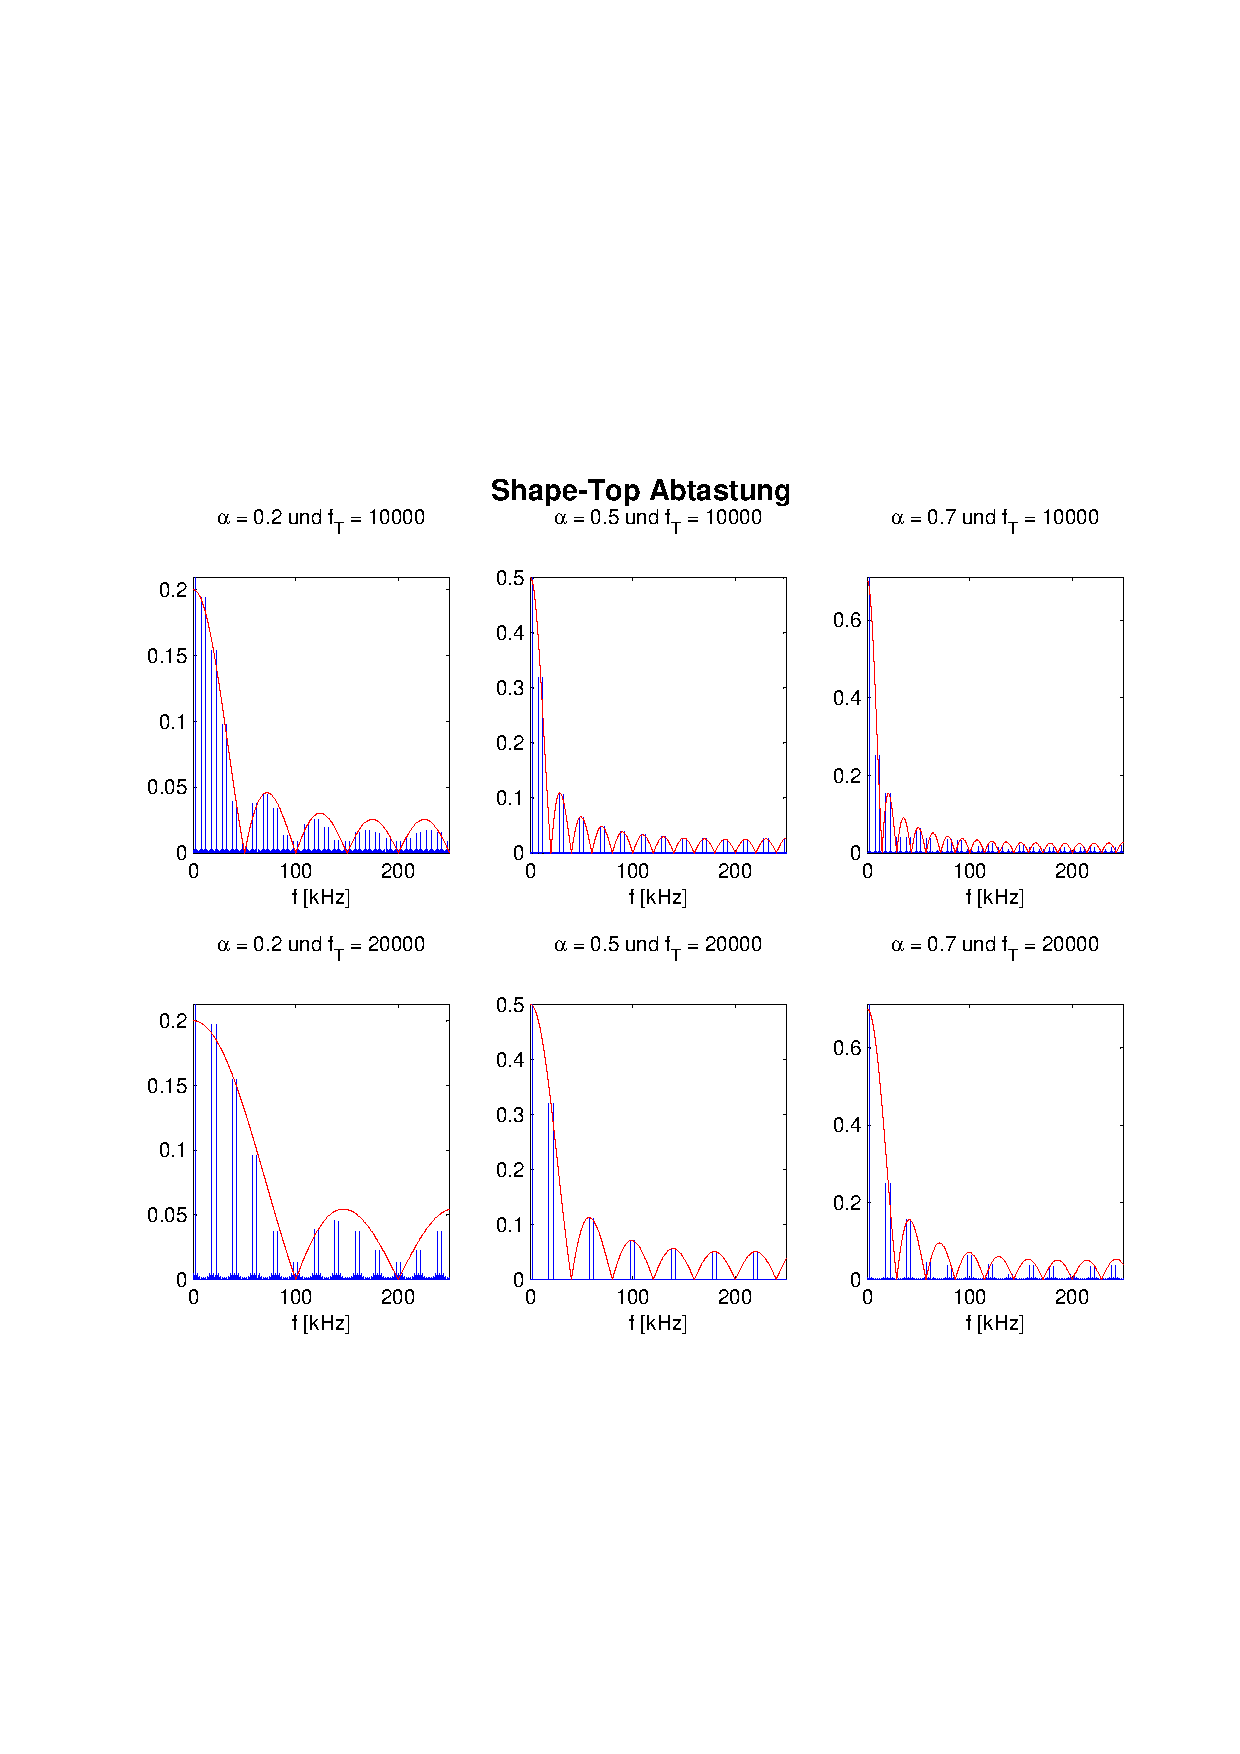
\includegraphics[scale=0.7, trim = 1.5cm 6cm 1cm 8cm,
        clip]{./Bilder/shape-top-freq_1V}
            \caption{Frequenzsignal mit shape-top-sampling und Abtastamplitude
            1V}
  	    \end{figure}
  	    
  	    Im Zeitsignal sieht man eine maximale Amplitude von $2V$, welche durch
  	    die Multiplikation von den $2V$ des Quellsignals und dem $1V$ des
  	    Abtastsignals entsteht. Die Form der Rechtecke nehmen oben den
  	    Sinusverlauf des Quellsignals an, was im Zeitsignal den Unterschied zu
  	    der flat-top Abtastung ausmacht. Zusätzlich kann man deutlich sehen, dass
  	    die Verdopplung der Abtastfrequenz ungefähr doppelt so viele abgetastete Stellen ergibt und 
  	    dass ein größeres Tastverhältnis die Breite der Dauer der Abtastung erhöht. 
  	    Als Umhüllende haben wir das Quellsignal verwendet.\\
  	    Im simmulierten Spektrum kann man erkennen, dass die Amplituden der
  	    drei Basisbänder für die drei Tastverhältnisse exakt dem eingesetzten
  	    Tastverhältnis $\alpha$ mal $1V$ entsprechen. Mit wachsender Frequenz
  	    nehmen die Peaks deutlich an Amplitude ab. Außerdem kann man sehen, dass
  	    die auftretenden Peakpaare immer die gleiche Amplitude besitzen. Dieses
  	    unverzerrte Spektrum war bei einer shape-top Abtastung zu erwarten.
  	    Die Umhüllende des Spektrums ist eine Si-Funktion.
  	    
    	Wenn man nun die Amplitude des Abtastsignals erhöht, erhält man folgende
    	Plots:
    	
    	\begin{figure}[H]
        \centering
        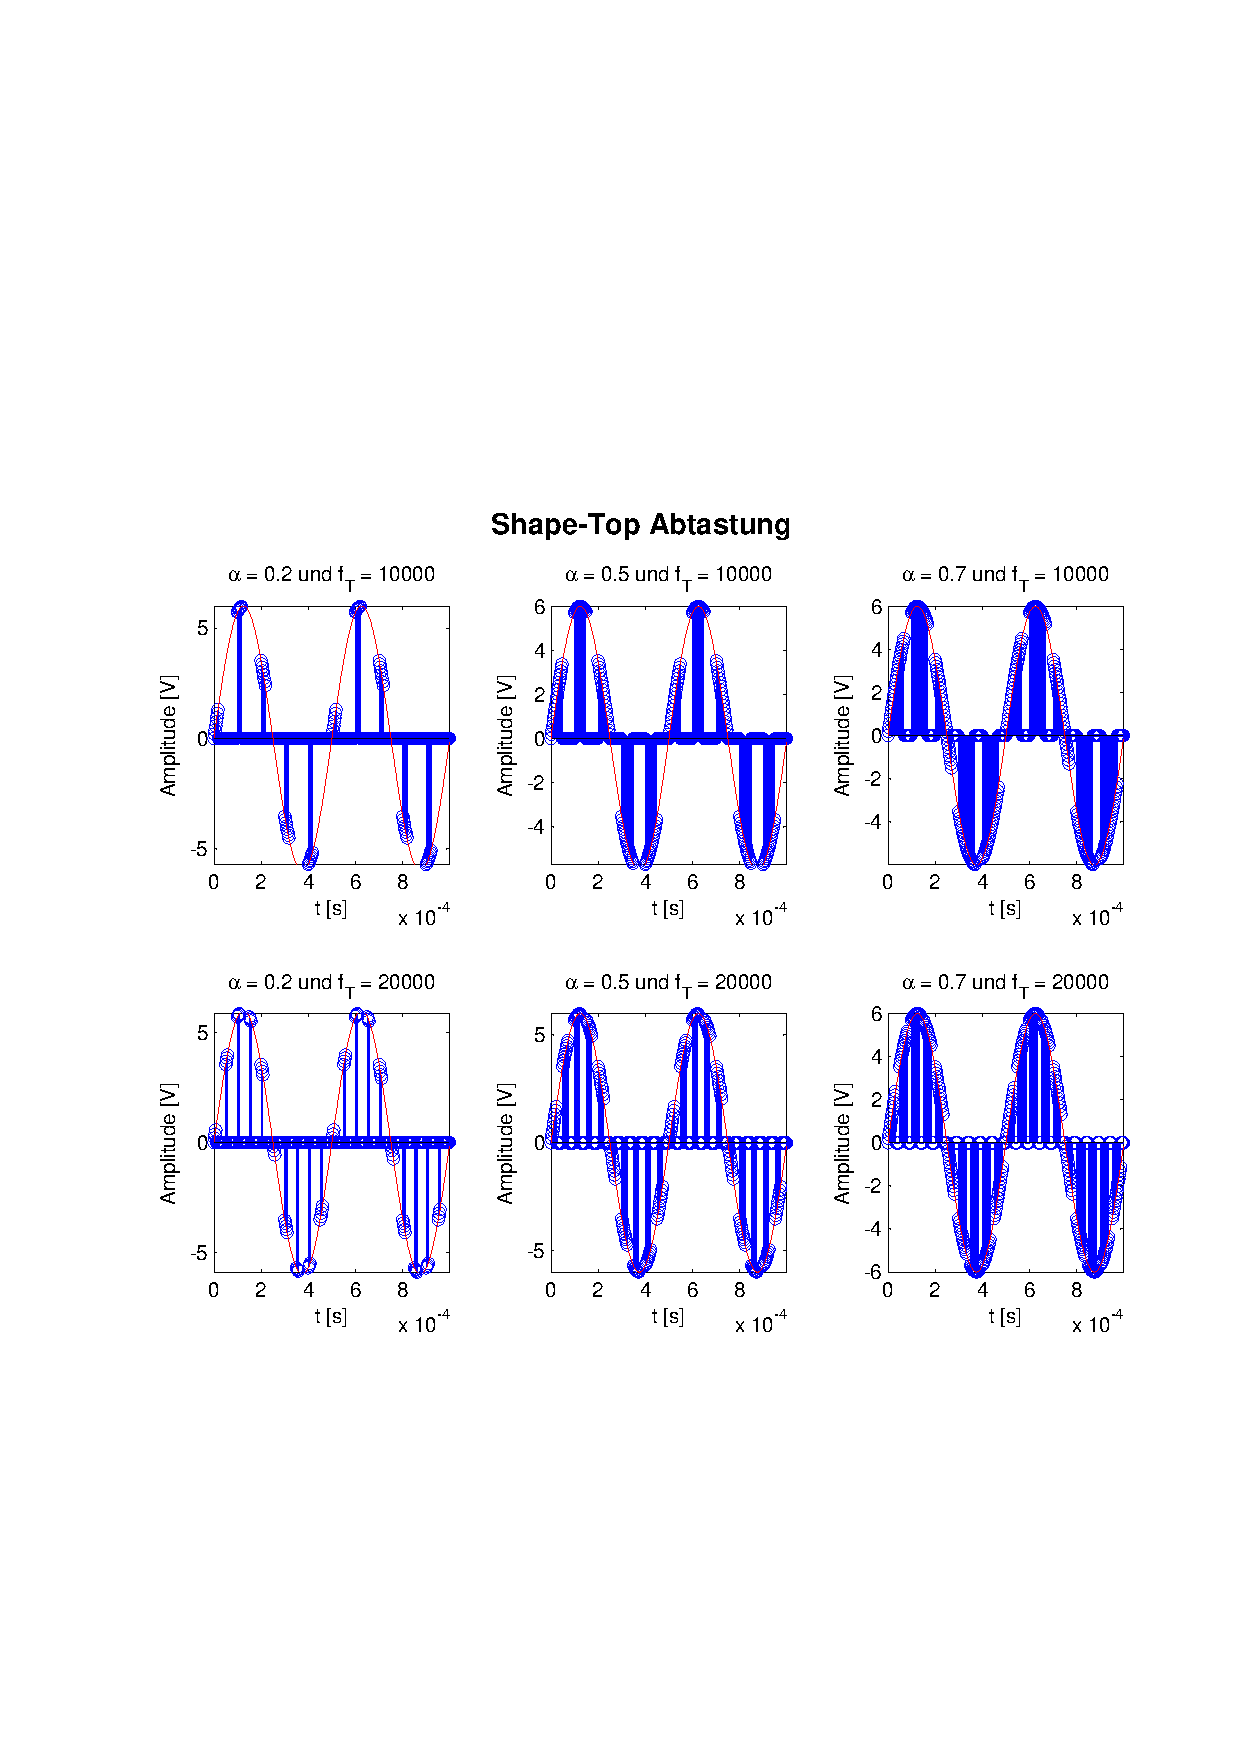
\includegraphics[scale=0.7, trim = 1.5cm 6cm 1cm 8cm,
        clip]{./Bilder/shape-top-zeit_3V}
            \caption{Zeitsignal mit shape-top-sampling und Abtastamplitude 3V}
  	    \end{figure}
  	    
  	    
  	    \begin{figure}[H]
        \centering
        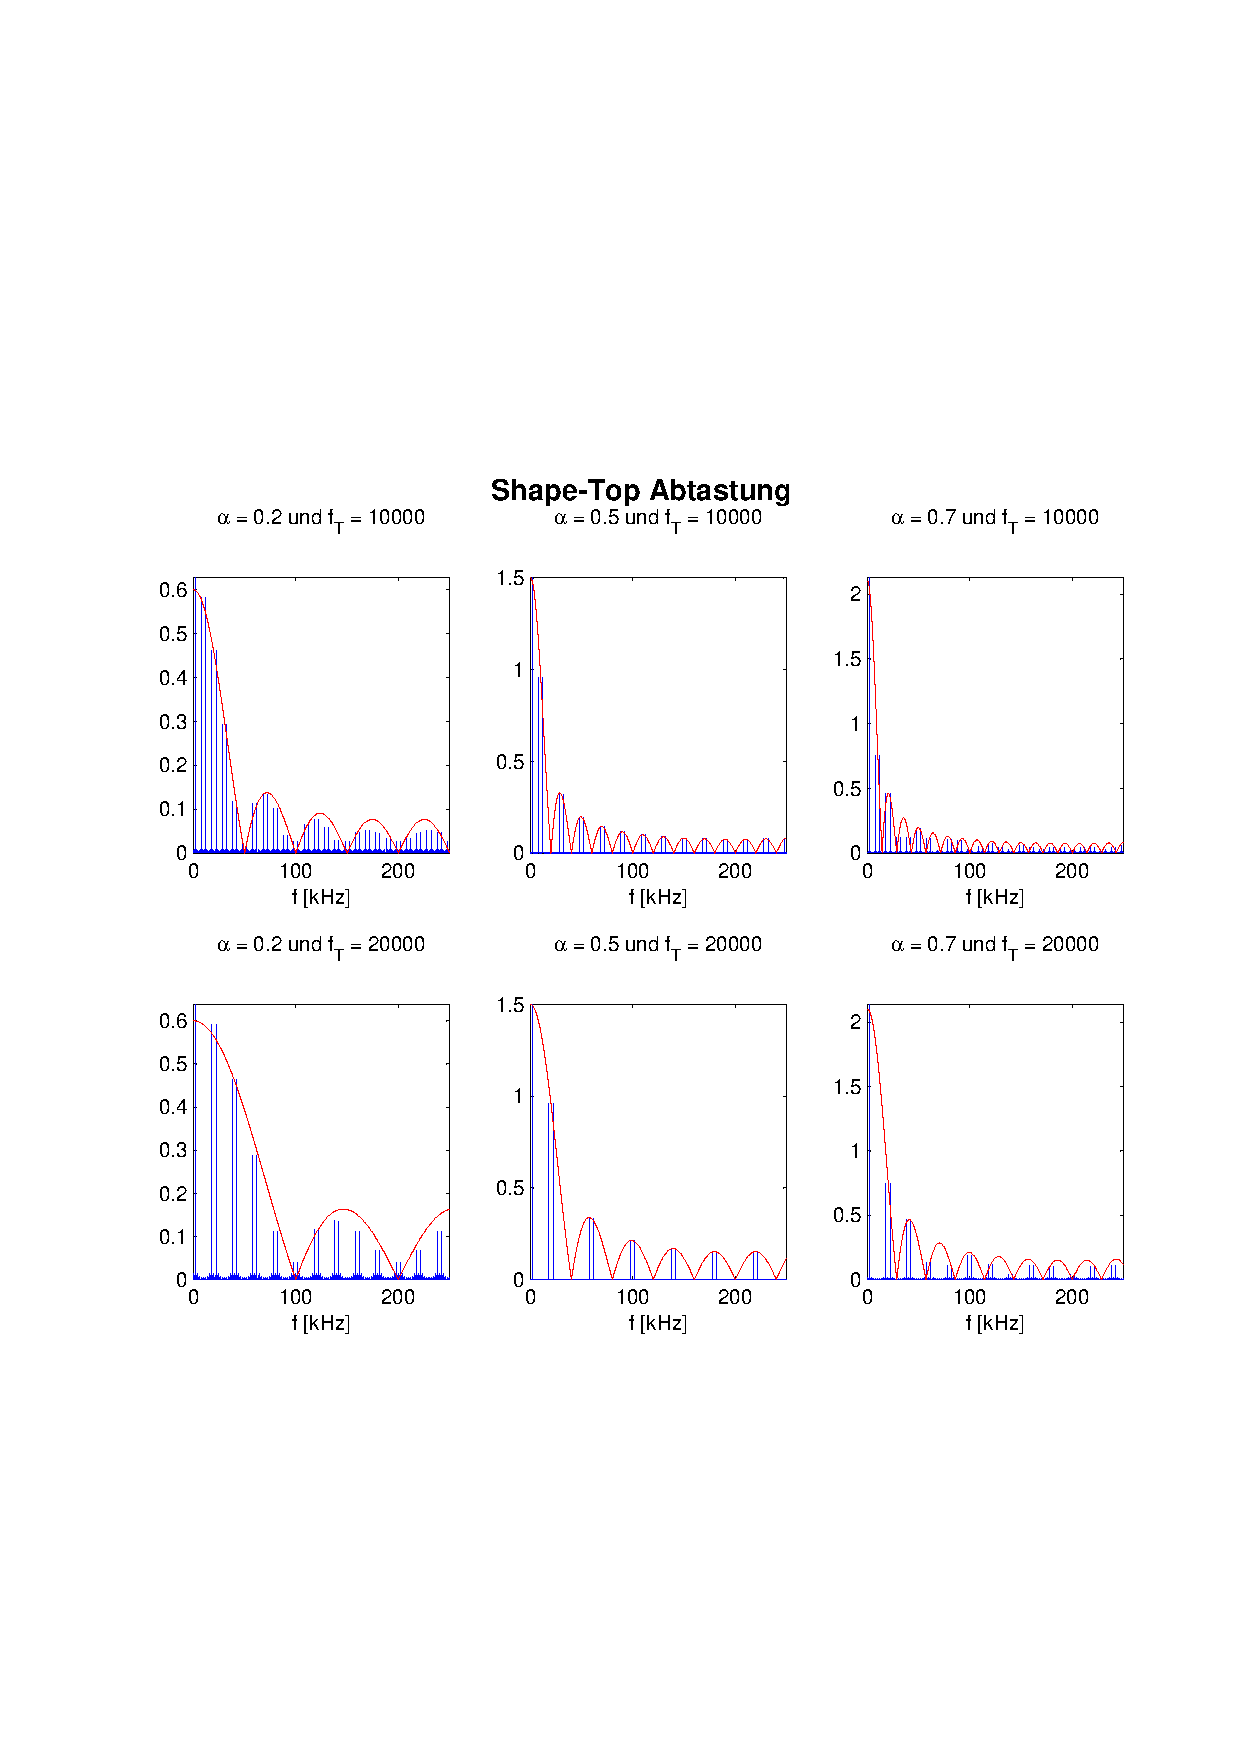
\includegraphics[scale=0.7, trim = 1.5cm 6cm 1cm 8cm,
        clip]{./Bilder/shape-top-freq_3V}
            \caption{Frequenzsignal mit shape-top-sampling und Abtastamplitude
            3V}
  	    \end{figure}
  	    
  	    
  	    Im Zeitsignal beträgt die Amplitude diesmal $6V$, welche durch die
  	    Multiplikation von $2V \cdot 3V$ entsteht. Alle anderen Auswirkungen der
  	    Tastfrequenz und des Tastverhältnisses bleiben gleich.\\
  	    Auch im Spektrum liegt der einzige Unterschied in den Maximalamplituden,
  	    welche nun um den Faktor $3$ (durch die $3V$ Amplitude des Abtastsignals)
  	    größer sind.
  	    
  	    \vspace{1em}
  	    
  	    Nun betrachten wir die Simmulationsergebnisse der Abtastung mit
  	    Signalverbreiterung:
  	    
  	    \begin{figure}[H]
    \centering
        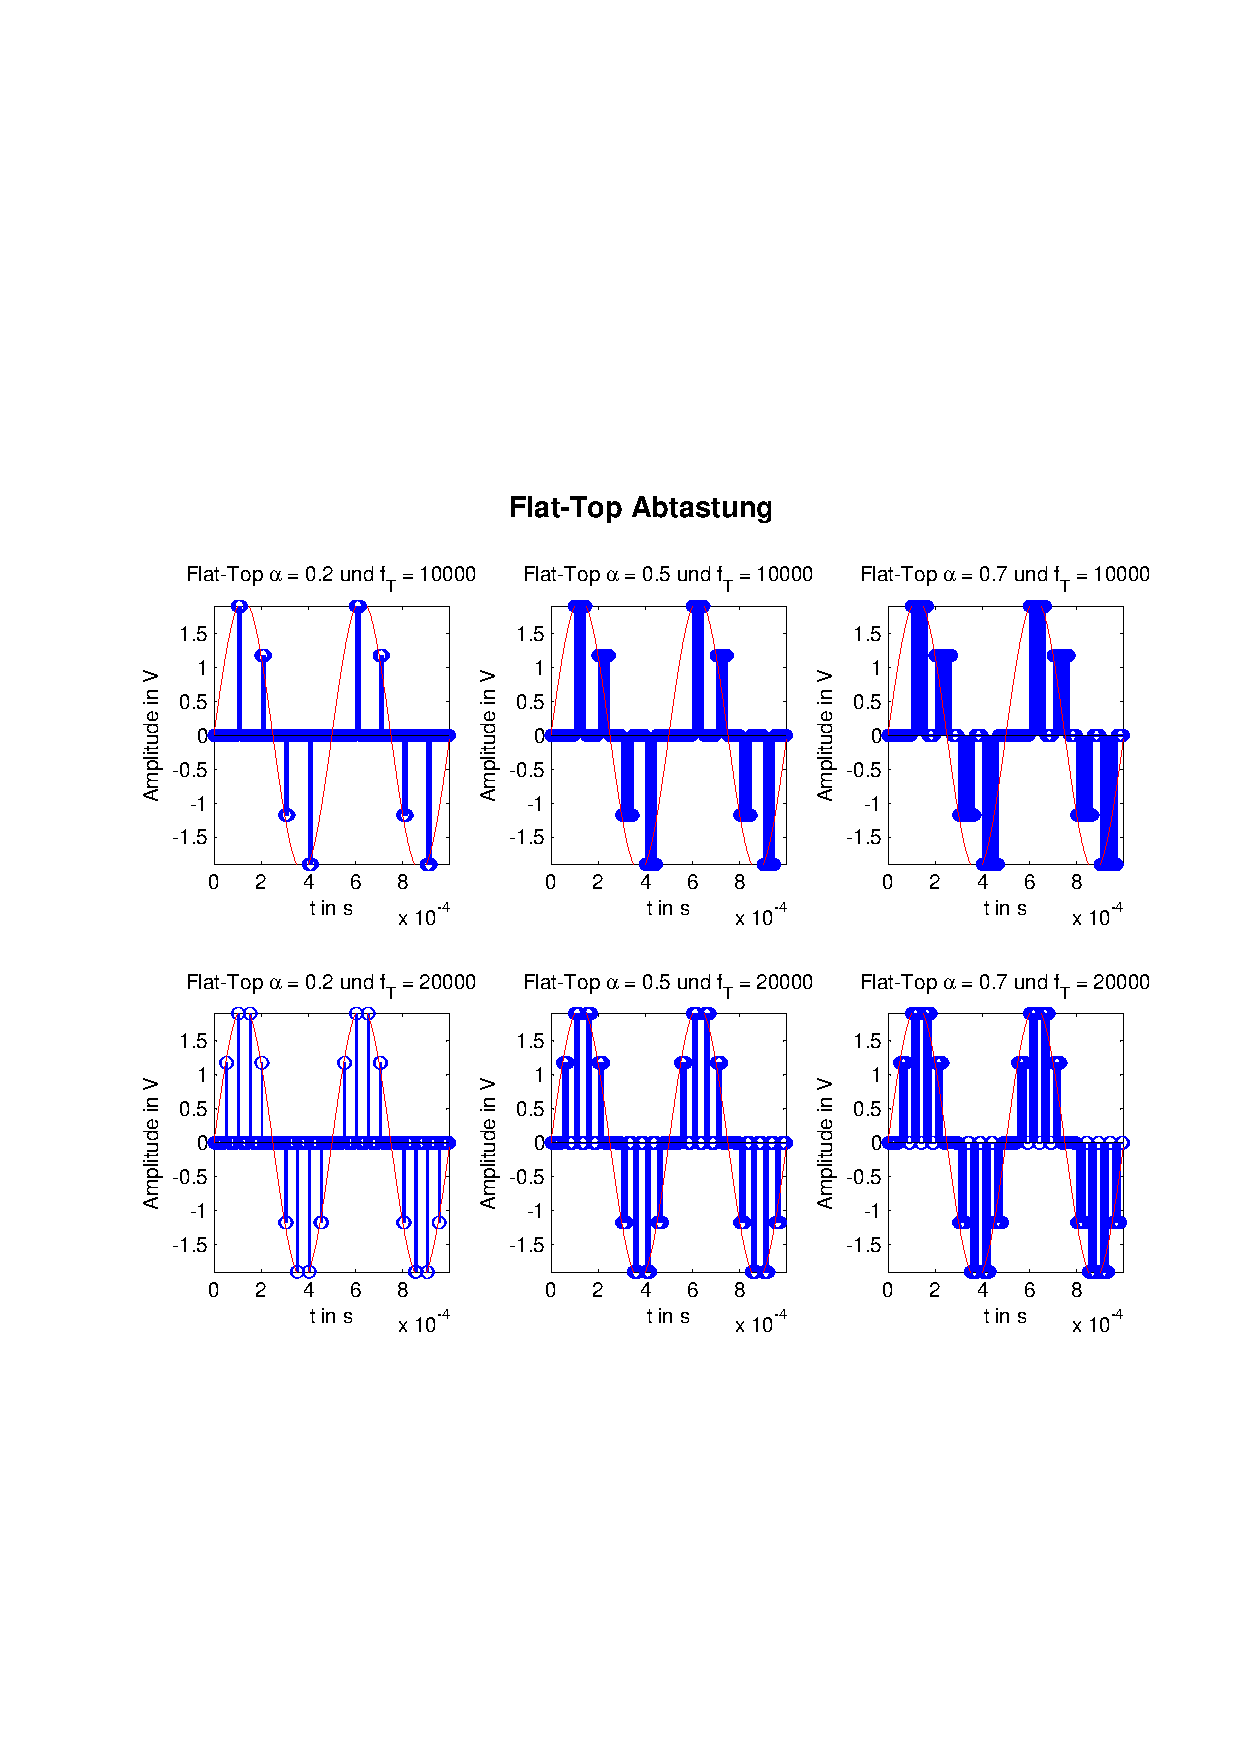
\includegraphics[scale=0.7, trim = 1.5cm 6cm 1cm 8cm,
        clip]{./Bilder/flat-top-zeit_1V}
            \caption{Zeitsignal mit flat-top-sampling und Abtastamplitude 1V}
  	    \end{figure}
  	    
  	    
  	    \begin{figure}[H]
    \centering
        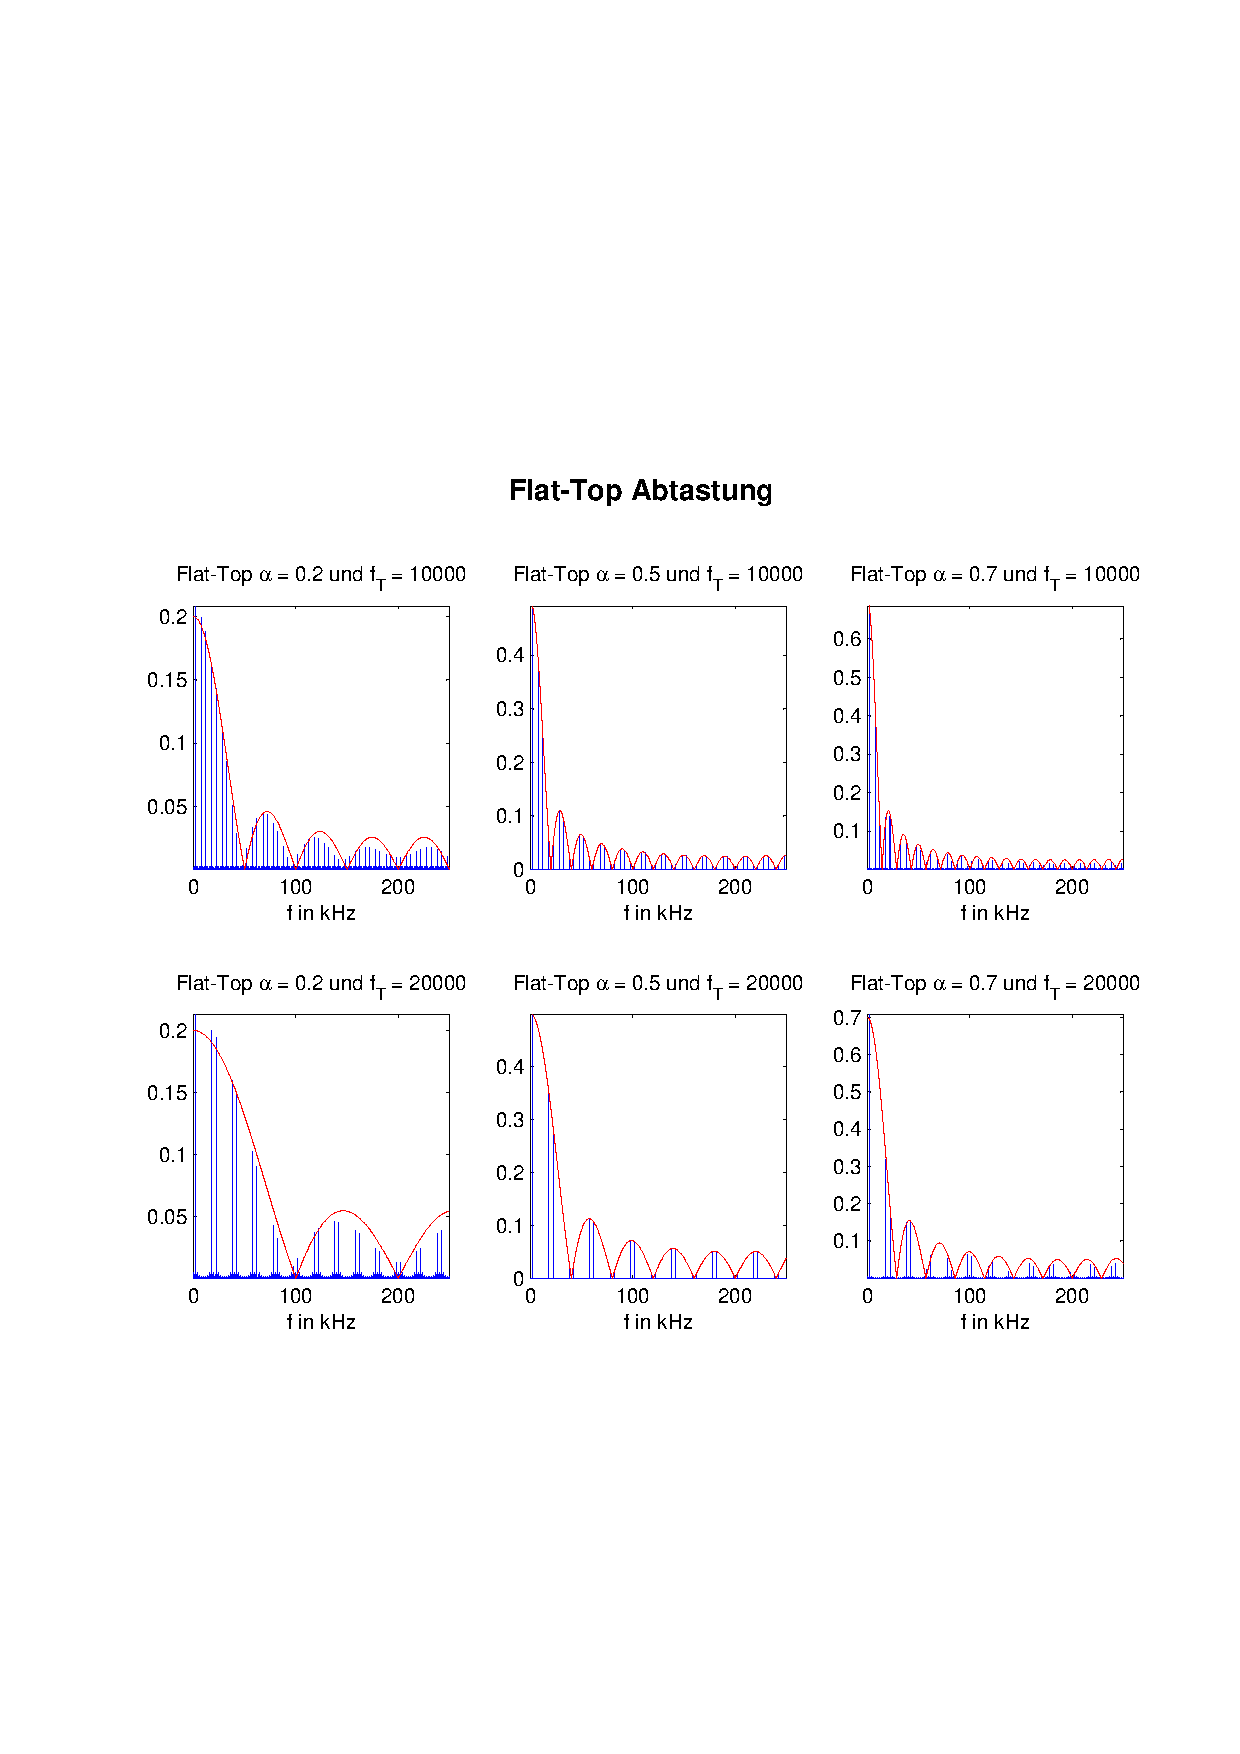
\includegraphics[scale=0.7, trim = 1.5cm 6cm 1cm 8cm,
        clip]{./Bilder/flat-top-freq_1V}
            \caption{Frequenzsignal mit shape-top-sampling und Abtastamplitude
            1V}
  	    \end{figure}
  	    
  	    Die Amplituden, die Breiten und die Häufigkeiten der abgetasteten Stellen
  	    stimmen bei der flat-top Abtastung mit den Werten des Zeitsignals der
  	    shape-top Abtastung überein. Der einzige Unterschied, den man wie erwartet sehen
  	    kann, ist, dass die Rechtecke sich nicht dem Sinusverlauf anpassen
  	    sondern ab der Abtaststelle die Sinusamplitude annehmen und durch das
  	    Hold-Glied über die Dauer der Abtastung behalten. Daher sind diese
  	    Rechtecke oben flach.\\
  	    Durch die DFT dieser Rechtecke aus dem Zeitsignal entstehen in dem
  	    Spektrum Peaks mit frequenzabhängiger Amplitude, die deutlich
  	    besser in die umhüllende Si-Funktion passen, als das Spektrum einer
  	    shape-top Abtastung. Ansonsten verhält sich das Spektrum im Bezug auf
  	    Tastfrequenz und -verhältnis nicht anders als bei der Abtastung durch
  	    Signalausblendung.
  	    
  	    Nun wird wieder die Abtastamplitude erhöht:
  	    
  	    
  	    \begin{figure}[H]
    \centering
        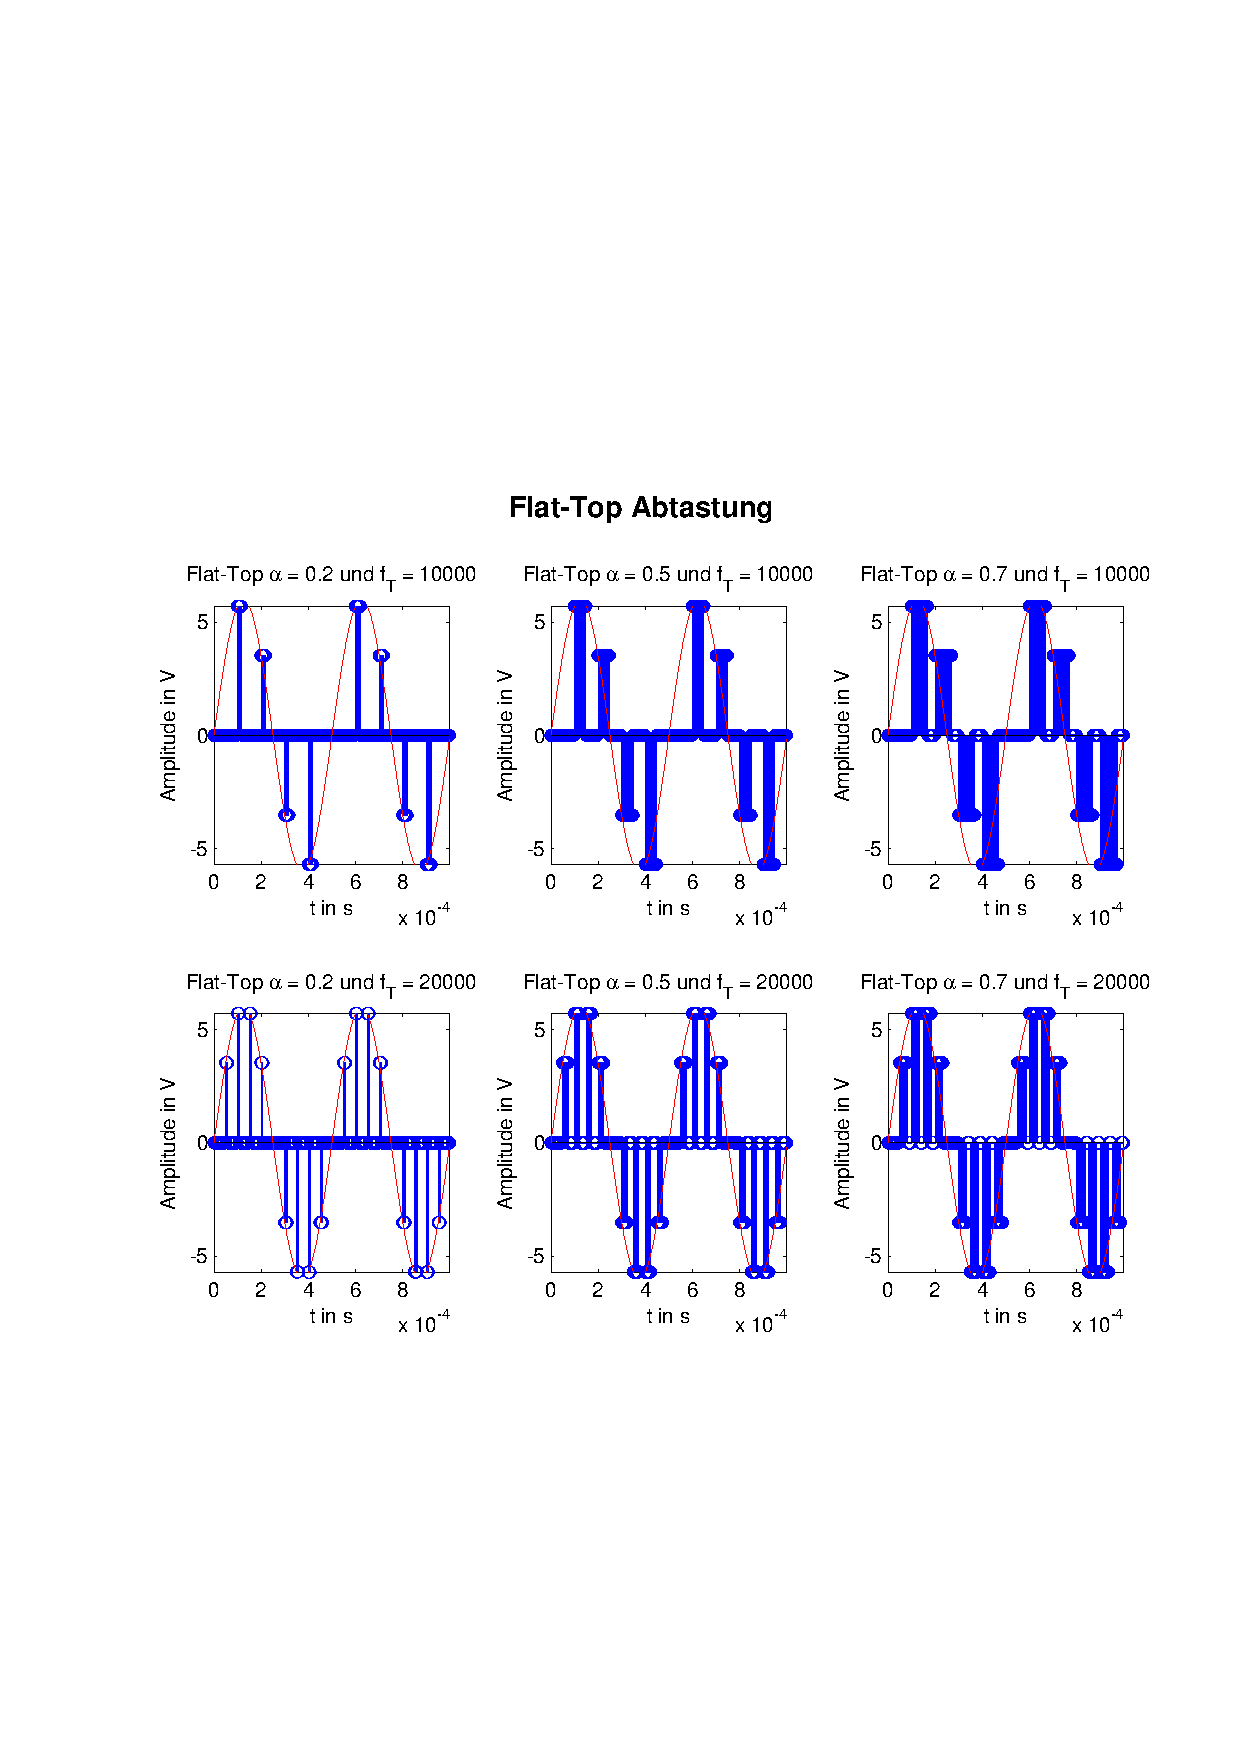
\includegraphics[scale=0.7, trim = 1.5cm 6cm 1cm 8cm,
        clip]{./Bilder/flat-top-zeit_3V}
            \caption{Zeitsignal mit flat-top-sampling und Abtastamplitude 3V}
  	    \end{figure}
  	    
  	    
  	    \begin{figure}[H]
    \centering
        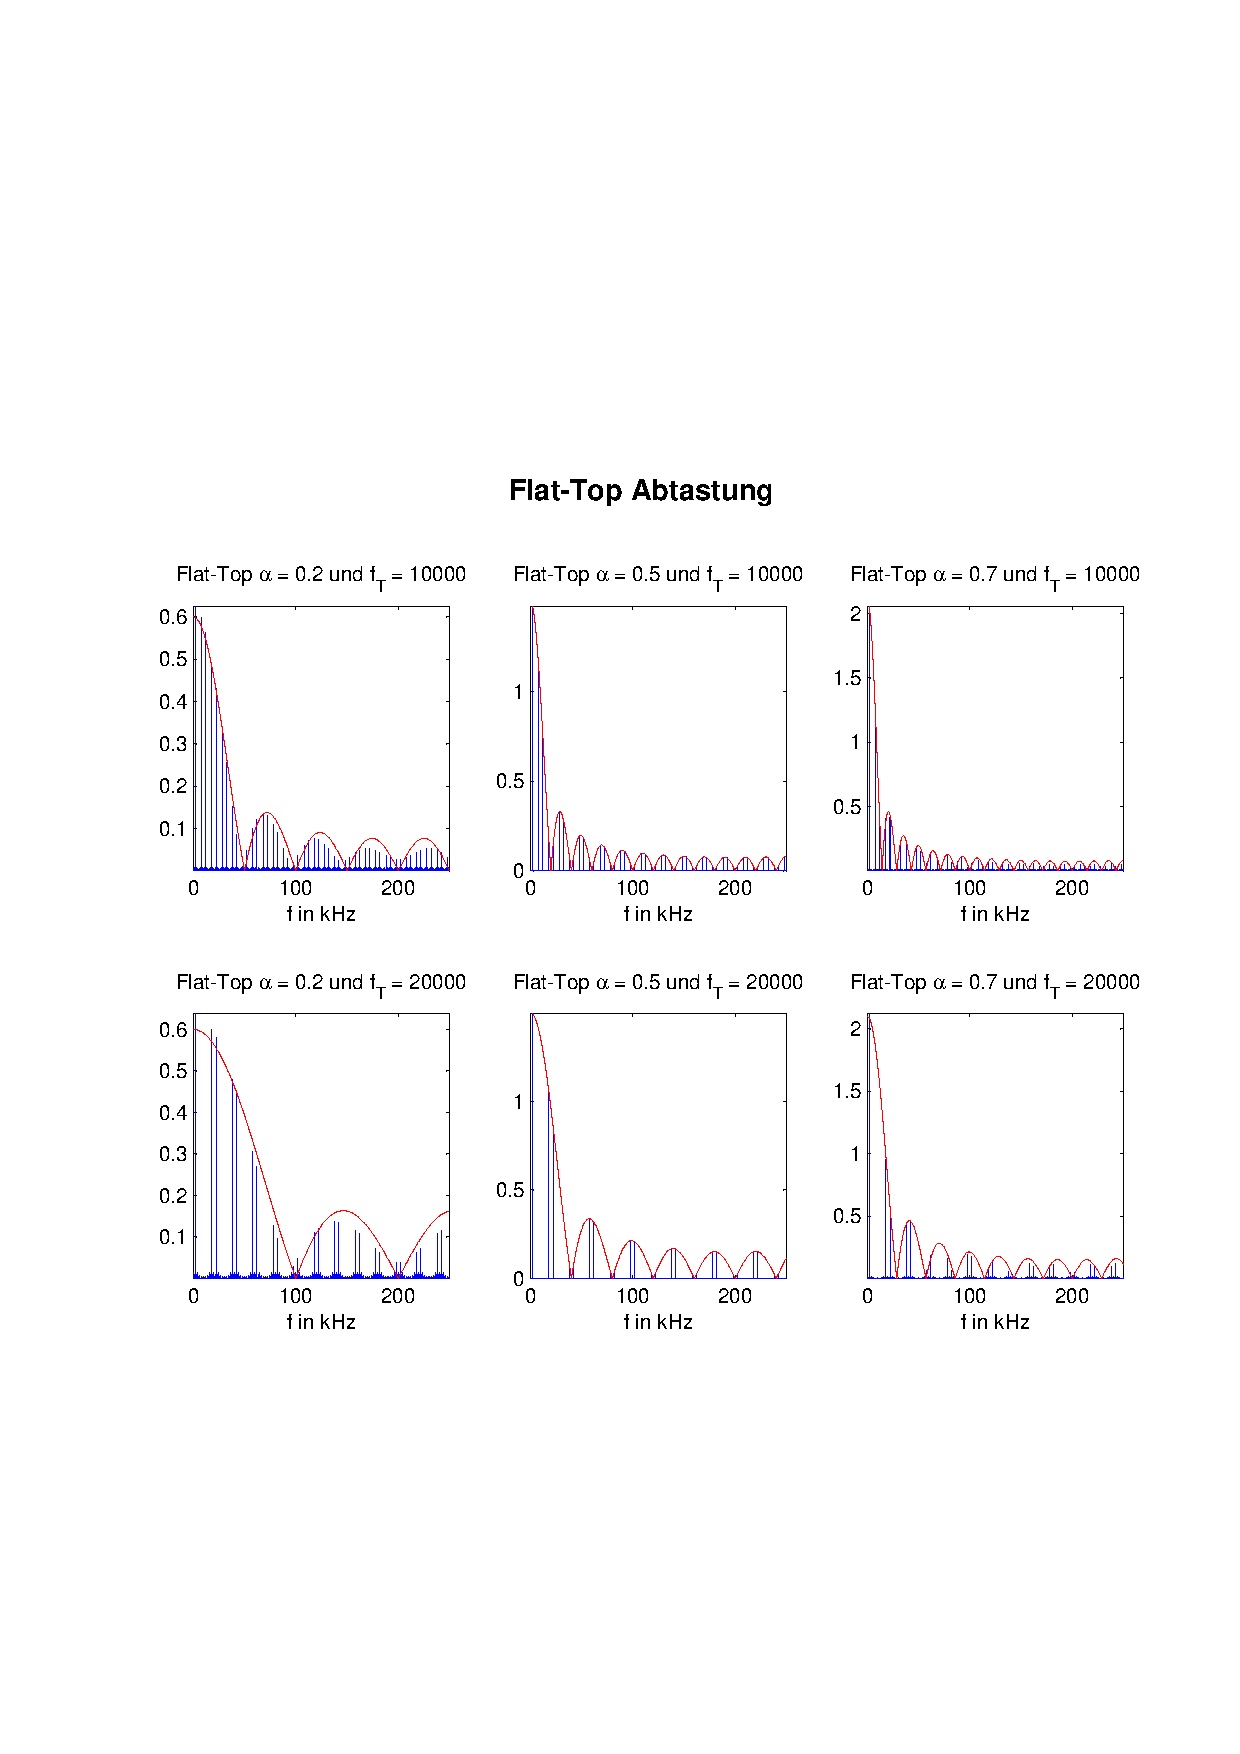
\includegraphics[scale=0.7, trim = 1.5cm 6cm 1cm 8cm,
        clip]{./Bilder/flat-top-freq_3V}
            \caption{Frequenzsignal mit flat-top-sampling und Abtastamplitude
            3V}
  	    \end{figure}
  	    
  	    
  	    Die Amplituden im Zeitsignal betragen wieder $6V$ und die Amplituden der
  	    Basisbänder nehmen die Werte $3V \cdot \alpha$ an. Ansonsten ist das
  	    Spektrum erneut deutlich verzerrter und alle anderen erwarteten
  	    Ergebnisse können auch hier wahrgenommen werden.
  	    
  	    
    \TODO{sind die Vorbereitungsaufgaben gut genug, dass wir sie beenden
    können?} 
    
    \end{quote}%subsection beenden

\end{quote}%Theorie beeanden
    
    \section{Labordurchführung}
    \begin{quote}
         \TODO{Durchführung schreiben}
   	\end{quote}%beende Labordurchführung
    	    
    
    \section{praktische Umsetzung}
    \begin{quote}
    Die praktische Umsetzung des Versuchs ist für beide Abtastverfahren gleich.
    
    \TODO{zu Ende bringen}
    \end{quote}%beende praktische Umsetzung
    
    
    \section{Auswertung}
    \begin{quote}    
        \TODO{Auswertung schreiben}
    \end{quote}%beende Auswertung
    
    \section{Zusammenfassung}
    \begin{quote}
    	\TODO{Zusammenfassung schreiben}
    \end{quote}%beende Zusammenfassung

%--------------------------------------------------------------------
%--------------------------------------------------------------------            

\TODO{Boris: öfter mal ein Überraschungsgeschenk für deine beste Freundin
besorgen!!}

%--------------------------------------------------------------------
%--------------------------------------------------------------------    


\begin{thebibliography}{999}
% \bibitem {AMohnetraeger} Prof. Dr.-Ing. Sikora, Thomas; Prof. Dr.-Ing. Noll, Peter: Einführung in die
% Nachrichtenübertragung, S.207




%Name, Vorname.; evtl. Name2, Vorname2.: Titel des Dokumentes
%oder Buches, Zeitschrift/Verlag/URL (Auflage, Erscheinungsort, -jahr), ggf. Seitenzahlen
% \bibitem {PasevalscheTheorem} \url{https://de.wikipedia.org/wiki/Parsevalsches_Theorem}, Zugriff
% 23.05.2012
\end{thebibliography}

\end{document}
